\documentclass[12pt]{article}
\usepackage[utf8]{inputenc}
\usepackage{hyperref}
\usepackage{graphicx}
\graphicspath{ {img/} }
\usepackage[justification = centering]{caption}
\usepackage{float}
\usepackage{amsmath}
%\usepackage[version=4]{mhchem}
\usepackage{booktabs} % nice rules (thick lines) for tables
\usepackage{microtype} % improves typography for PDF
\usepackage{float}
\usepackage{multicol}

\newcommand{\labname}{458 Group 8 Nuclear Shipping\xspace}%

%\course{NPRE 448}
\title{Nuclear-powered Shipping}
\author{Louis Kissinger, Brad Ellis, and Adam Pichman \\Course: NPRE 458; Advisor: Magdi Ragheb}
\date{February 22, 2019}
\makeatletter
\setlength{\@fptop}{0pt}
\makeatother

\begin{document}

%TITLE PAGE
\maketitle
%
\pagebreak
%ABSTRACT
\begin{abstract}
Nuclear power was analyzed as an alternative to fossil fuel combustion for propulsion of large boats. In particular, ... 
\end{abstract} 

\pagebreak
\tableofcontents

%\begin{multicols}{2

%%%%%%%%%%%%%%%%%%%%%%%%%%%%%%%%%%%%%%%%%%%%%%%%%%%%%%%%%%%%%%%%%%%%%%%%%%%%%%%%
\section{Introduction}
Introduction

If you wanna cite Alekseev put \cite{alekseev}

If you wanna cite Carlton put \cite{Carlton}

\cite{Gravina}

\cite{Han}

\cite{iaea}

If you wanna cite Hirdaris put \cite{Hirdaris}

If you wanna cite Jacobs put \cite{Jacobs}

If you wanna cite Holtec put \cite{Holtec}



%%%%%%%%%%%%%%%%%%%%%%%%%%%%%%%%%%%%%%%%%%%%%%%%%%%%%%%%%%%%%%%%%%%%%%%%%%%%%%%%
\section{Background and State of the Art}
Background and state of the art
%%%%%%%%%%%%%%%%%%%%%%%%%%%%%%%%%%%%%%%%%%%%%%%%%%%%%%%%%%%%%%%%%%%%%%%%%%%%%%%%
\section{Conceptual Design}
\subsection{Naval concept}
\subsubsection{Oceanic tug boat}
\subsubsection{Offshore power plant and coastal tug boat}
\subsection{Reactor concept}
\subsubsection{Core concept}
\subsubsection{Neutronics analysis}
The following analysis determines the enrichment required to reach $k_\infty = 1$:

\begin{align}
k_\infty &= \eta f = 1 \\
 &= \nu \frac{\sigma_f^F}{\sigma_a^F} \frac{\Sigma_a^F}{\Sigma_a} \label{e:kinfty}
\end{align}

Approximate values of these parameters are given in table \ref{t:jaea-table}.

\begin{table}[H]
\begin{center}
  \caption{Approximate values of nuclear properties germaine to equation \ref{e:kinfty}, \cite{jaea}}
  \label{t:jaea-table}
  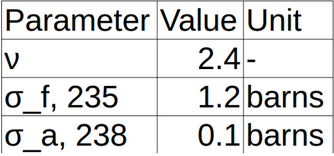
\includegraphics[width=0.5\textwidth]{full-spectrum-nuke-data}
\end{center}
\end{table}


The macroscopic cross section is by definition $\Sigma = N \sigma = \frac{\rho N_{av}}{A} \omega$. Equation \ref{e:kinfty} then reduces to:

\begin{align}
1 &= \nu \frac{^{235}\sigma_f}{^{235}\sigma_a} \frac{\frac{\omega}{235} ^{235} \sigma_a}{\frac{1 - \omega}{238} ^{238} \sigma_a} \\
 &= \nu \frac{^{235} \sigma_f}{^{238} \sigma_a} \frac{238 \omega}{235 (1 - \omega)} 
\end{align}

Upon defining a new variable $\xi = \nu \frac{^{235} \sigma_f}{^{238} \sigma_a}$, we find:

\begin{align}
\frac{1}{\xi} &= \frac{238 \omega}{235 (1 - \omega)} \\
\omega &= \frac{235}{238 \xi + 235} < 1
\end{align} 

Upon inserting the tabulated values for these cross sections, we find $\xi = 4.2$ and $\omega = 0.0336 = 3.4 \% $. The bulk of the reactor can thus be fueled without HEU.

\textbf{If the fuel is $UO_2$}, then the mass of Uranium per mass of fuel is:

\begin{align}
\frac{m_U}{m_{UO2}} &= \frac{238 (1 - \omega) + 235 \omega}{238 (1 - \omega) + 235 \omega + 32} \\
 &= 0.8817 \frac{grams}{gram}
\end{align}
It is now easy to find the number of $U_{235}$ atoms per gram of fuel:
\begin{align}
n_{235} &= \omega \frac{m_u}{m_{UO_2}} \frac{N_{av}}{235} \\
 &= 7.906 \times 10^{21}
\end{align}

If we \textbf{assume that $\frac{3}{4}$ of the fissions occur in $U_{235}$}, then the total fissile atoms per gram of fuel is $1.05 \times 10^{21}$. 

We can now determine the required mass of Uranium to produce a certain amount of energy. The core's power is related to the fission rate by a factor of 200 MeV per fission. We will \textbf{assume a core power of .175 GWth} for this analysis. This value roughly corresponds to 50 MWe for typical values of efficiency, which is close to the power output of the reactors we seek to imitate. The fission rate in our reactor is then $1.75 \times 10^8 \frac{Joules}{sec} \times \frac{1 MeV}{1.6 \times 10^{-13} Joules} \times \frac{1 Fission}{200 MeV} = 5.5 \times 10^{18} \frac{fissions}{second}$. Now consider a \textbf{2 year refueling cycle}, which requires $5.5 \times 10^{18} \frac{fissions}{second} \times \frac{6.3 \times 10^7 s}{2 years} = 3.5 \times 10^{26} \frac{fissions}{cycle}$.

Returning to our value of fissile atoms per gram of $UO_2$, we can find the mass of Uranium required to power our core for two years. Recall that we anticipate $1.05 \times 10^{21}$ fissile nuclei per gram of fuel. The mass of fuel needed is then $\frac{3.5 \times 10 ^{26}}{1.05 \times 10^{21}} = 2.90 \times 10^{5} g = 290 kg$. However, we do not expect to burn every fissile isotope, \textbf{so this value should be adjusted by a factor of 1.7}, so that our first estimate of the mass of fuel is 493 kg. 

The density of $UO_2$ is $10970 \frac{kg}{m^3}$. The Volume of this much fuel is therefore $V = \frac{493 kg}{10970 \frac{kg}{m^3}} =  0.45 m ^ 3 $

\textbf{We will assume that the volume of our cylindrical core is equal to the volume of a cylinder of the same radius, which is to say $H = \frac{4}{3} R$}. Under this assumption, the radius of our core is $(\frac{3}{4} \pi V) ^ {1/3} = 1.07 meters,$ giving a height of $1.43 meters$. This first estimate of the height (which will most likely be shorter than the final value) will be very useful in the thermal analysis.   
\subsubsection{Thermal analysis}
Let us begin by estimating the mass flow rate required to remove the fission heat at steady state. With a simple energy balance, it becomes apparent that heat flux is related to the heat capacity and mass flow rate of the coolant and the temperature change across the length of the channel as follows:

\begin{align}
q'' &= \dot{m} c_p \Delta T \\
\dot{m} &= \frac{q''}{c_p \Delta T}
\end{align}

We can estimate q'' by dividing the thermal power by the surface area of the fuel, which gives us $q'' = \frac{1.5 \times 10^8}{2 \pi N 1.43 \times 10 ^{-2}}$ if there are N fuel rods, each with 1-cm radius and 1.43 meters tall. For this preliminary analysis, \textbf{we will assume 100 rods}. It then follows that the heat flux from such a system is $1.67 \times 10^7 \frac{w}{cm^2}$. 

Our coolant, Lead-Bismuth Eutectic, is liquid between approximately 200-1670 Degrees C. Conservatively, the $\Delta T$ may then approach 1,000 Kelvin. The isobaric heat capacity of this fluid in this temperature range is approximately $130 \frac{J}{kg K}$ \cite{LBE_properties}. The Mass flow rate needed is therefore:

\begin{align}
\dot{m} &= \frac{q''}{c_p \Delta T} \\
 &= \frac{1.67 \times 10^7 \frac{w}{cm^2}}{130 \frac{J}{kg K} \times 1000} = 131 \frac{kg}{s}
\end{align} 

Dividing this flow rate by the density of LBE gives an approximate mass flow rate of 0.015 $\frac{m^3}{s}$.

\subsubsection{Materials analysis}
\subsubsection{Alternatives}
Conceptual design
%%%%%%%%%%%%%%%%%%%%%%%%%%%%%%%%%%%%%%%%%%%%%%%%%%%%%%%%%%%%%%%%%%%%%%%%%%%%%%%%
\section{Conclusions}
Conclusions

%%%%%%%%%%%%%%%%%%%%%%%%%%%%%%%%%%%%%%%%%%%%%%%%%%%%%%%%%%%%%%%%%%%%%%%%%%%%%%%%

%%%%%%%%%%%%%%%%%%%%%%%%%%%%%%%%%%%%%%%%%%%%%%%%%%%%%%%%%%%%%%%%%%%%%%%%%%%%%%%%
\section{Acknowledgements}
Thanks to the Illinois NPRE department for their tireless work educating us. In particular, we would like to thank Professor Ragheb for his guidance and mentorship and Professor Stubbins for instructing the Senior Design course.

%%%%%%%%%%%%%%%%%%%%%%%%%%%%%%%%%%%%%%%%%%%%%%%%%%%%%%%%%%%%%%%%%%%%%%%%%%%%%%%%
\bibliographystyle{ans}
\bibliography{bibliography}
%\end{multicols}
\end{document}

